\documentclass[12pt]{article}
\usepackage[russian]{babel}
\usepackage[utf8x]{inputenc}
\usepackage{amssymb}
\usepackage{amsmath}
\usepackage{graphicx}
\usepackage[margin=.7in]{geometry}
\usepackage[colorinlistoftodos]{todonotes}
\usepackage{listings}
\usepackage[section]{placeins}
\usepackage[T1]{fontenc}
\usepackage{float}
\usepackage{url}
\newcommand\purl[1]{\protect\url{#1}} % "protected url"

\usepackage[section]{placeins}
\let\Oldsection\section
\renewcommand{\section}{\FloatBarrier\Oldsection}

\let\Oldsubsection\subsection
\renewcommand{\subsection}{\FloatBarrier\Oldsubsection}

\let\Oldsubsubsection\subsubsection
\renewcommand{\subsubsection}{\FloatBarrier\Oldsubsubsection}
\begin{document}

\title{Оценка параметров систем массового обслуживания}
\author{Андрей Валиков}
\date{}
\maketitle

\section{Цель работы}
Оценить следующие характеристики коммутаторов: вероятность потерь вызова, производительность, среднее число соединений. Лабораторная работа выполнена на языке Python 3.6 с использованием библиотек Matplolib и SciPy и представляет собой модели, позволяющие исследовать характеристики однозвенных коммутаторов при различных параметрах.

\section{Общая модель коммутатора}
Коммутатор в данной работе представляет собой модель, имеющую $M$ входов и $N$ выходов.

\begin{figure}[htp]
\centering
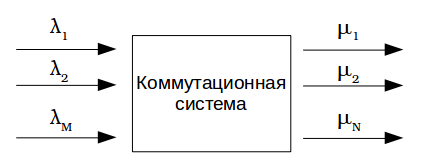
\includegraphics[scale=1.00]{assets/comm_model.png}
\end{figure}


\section{Параметры системы}\label{sec:systemParams}

\begin{tabular}{l l}
    $M$ & входы коммутатора \\
    $N$ & выходы коммутатора \\
    $\lambda$ & поступление нагрузки на одном входе \\
    $\mu$ & уход нагрузки с одного выхода \\
    $P$ & вероятность потерь вызовов \\
    $G$ & производительность \\
    $E$ & среднее число соединений \\
\end{tabular} \\
    $\rho = \frac{\lambda}{\mu}$ -- отношение поступления нагрузки к её уходу 

																																																							

\section{Вероятность блокировки для трёх распредлений}\label{sec:prob}


\subsection{Распределение Энгсета}\label{subsec:engset}

 \[
     p = \frac{\rho ^ N \binom{M}{N}}
     {\sum_{n=0}^{N} \rho ^ n \binom{M}{n}}
 \]

\subsection{Распределение Эрланга}\label{subsec:erlang}

\[
     p = \frac{(M \rho) ^ N}
     {N!\sum_{n=0}^{N + 1} \frac{(M \rho) ^ n}{n!}}
\]

\subsection{Биноминальное распределение}\label{subsec:binom}
Пусть $\alpha = \frac{\rho}{\rho + 1}$

\[
     p = \binom{M}{N} \alpha ^ N (1 - \alpha) ^ {M - N}
\]

\section{Код программы}

\subsection{\purl{main.py}}

\begin{lstlisting}
import math
import numpy as np
from queueing import Queueing
from mode_of_work import Mode

fact = math.factorial

mode = Mode.on_lambda

lam, mu = .9, .9


M, N = 10, 10

_range = np.arange(.01, 1, .05)


if mode == Mode.on_k:
    _range = np.arange(1, 20)

queueing = Queueing(lam, mu, M, N, _range, mode)

P1_k, G1_k, E1_k = [], [], []
P2_k, G2_k, E2_k = [], [], []
P3_k, G3_k, E3_k = [], [], []

for var in _range:

    if mode == Mode.on_lambda:
        queueing.lam, queueing.rho = var, var / mu
    elif mode == Mode.on_mu:
        queueing.rho = lam / var
    elif mode == Mode.on_rho:
        queueing.rho = var
    elif mode == Mode.on_k:
        queueing.N = var

    P1_k.append(queueing.p_engset())
    G1_k.append(queueing.perf(P1_k[-1]))
    E1_k.append(queueing.cons(P1_k[-1]))

    P2_k.append(queueing.p_erlang())
    G2_k.append(queueing.perf(P2_k[-1]))
    E2_k.append(queueing.cons(P2_k[-1]))

    P3_k.append(queueing.p_binom())
    G3_k.append(queueing.perf(P3_k[-1]))
    E3_k.append(queueing.cons(P3_k[-1]))

queueing.common_plot(
    title='loss_prob', title_eng='loss_prob',
    engset=P1_k, erlang=P2_k, binom=P3_k)
queueing.common_plot(
    title='perf', title_eng='perf',
    engset=G1_k, erlang=G2_k, binom=G3_k)
queueing.common_plot(
    title='aver_conn', title_eng='aver_conn',
    engset=E1_k, erlang=E2_k, binom=E3_k)

\end{lstlisting}

\subsection{\purl{mode_of_work.py}}
\begin{lstlisting}
from enum import Enum


class Mode(Enum):
    on_lambda = 0,
    on_mu = 1,
    on_rho = 2,
    on_k = 3
\end{lstlisting}

\subsection{\purl{queueing.py}}
\begin{lstlisting}
import matplotlib.pyplot as plt
import scipy.misc
import math
from mode_of_work import Mode
fact = math.factorial
comb = scipy.misc.comb


class Queueing:
    def __init__(self, lam, mu, M, N, _range, mode):
        self.lam, self.mu = lam, mu
        self.rho = lam / mu
        self.M, self.N = M, N
        self._range = _range
        self.mode = mode

    """Stage 1"""
    def p_engset(self):
        """engset loss probability"""
        _sum = sum((comb(self.M, n) * (self.rho ** n) for n in range(self.N + 1)))
        return comb(self.M, self.N) * ((self.rho ** self.N) / _sum)

    def p_erlang(self):
        """erlang loss probability"""
        _sum = sum(((self.M * self.rho) ** n) / fact(n) for n in range(self.N + 2))
        return (self.M * self.rho) ** self.N / (fact(self.N) * _sum)

    def p_binom(self):
        """binom loss probability"""
        alpha = self.rho / (1 + self.rho)
        return comb(self.M, self.N) * (alpha ** self.N) * (1 - alpha) ** (self.M - self.N)

    """Stage 2"""
    def perf(self, p):
        """performance"""
        return self.lam * self.M * (1 - p)

    """Stage 3"""
    def cons(self, p):
        """connections"""
        return self.rho * self.M * (1 - p)

    def common_plot(self, **kwargs):
        title = f"{kwargs['title']} "
        if self.mode == Mode.on_lambda:
            title += f'M={self.M} N={self.N} mu={self.mu}'
            plt.xlabel('lambda')
        elif self.mode == Mode.on_mu:
            title += f'M={self.M} N={self.N} lambda={self.lam}'
            plt.xlabel('mu')
        elif self.mode == Mode.on_rho:
            title += f'M={self.M} N={self.N} lambda={self.lam}'
            plt.xlabel('rho')
        elif self.mode == Mode.on_k:
            title += f'M={self.M} lambda={self.lam} mu={self.mu}'
            plt.xlabel('N')

    # file_title = f"_M{self.M}_N{self.N}_mu{self.mu}"

        plt.title(title)
        plt.plot(self._range, kwargs['engset'], label='Engset')
        plt.plot(self._range, kwargs['erlang'], label='Erlag')
        plt.plot(self._range, kwargs['binom'], label='Binom')
        plt.legend()
        # plt.savefig(file_title.replace('.', '') + '.png')
        plt.show()
\end{lstlisting}


\section{Задача 1. Зависимость параметров от $\lambda$}\label{sec:result}

\subsection{$M = N$}\label{subsec:}

\begin{figure}[!htb]
\centering
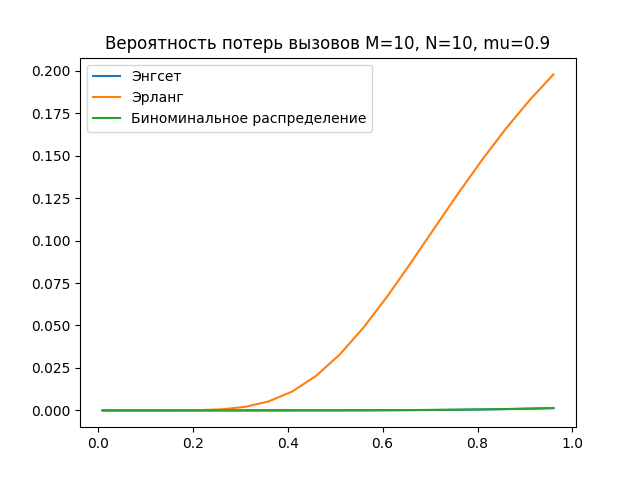
\includegraphics[scale=1.00]{assets/iss_1/loss_prob_M10_N10_mu09.png}
\caption{}
\label{}
\end{figure}

\begin{figure}[!htb]
\centering
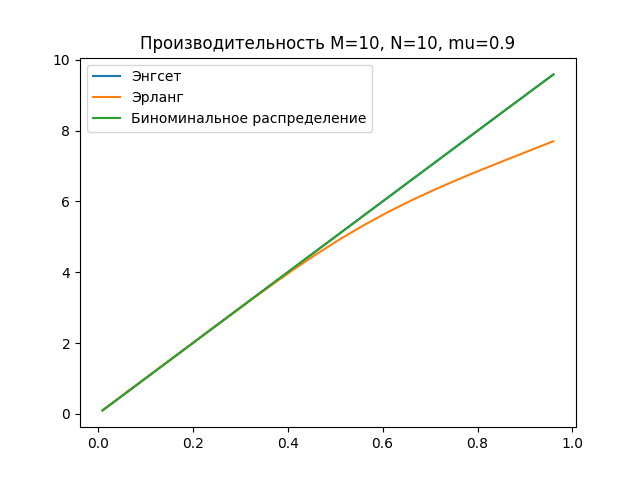
\includegraphics[scale=1.00]{assets/iss_1/perf_M10_N10_mu09.png}
\caption{}
\label{}
\end{figure}

\begin{figure}[!htb]
\centering
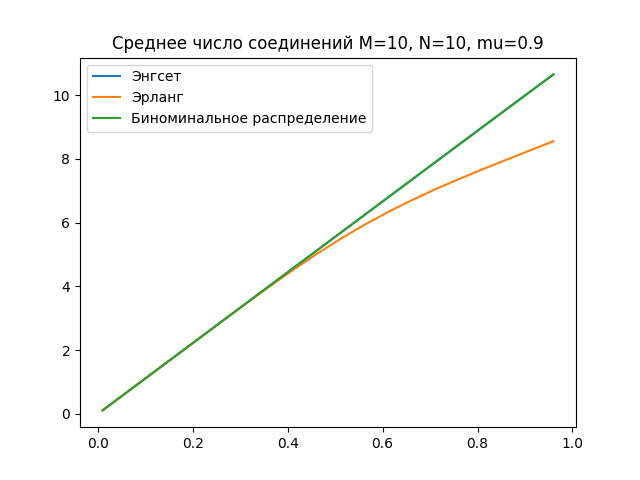
\includegraphics[scale=1.00]{assets/iss_1/aver_conn_M10_N10_mu09.png}
\caption{}
\label{}
\end{figure}

\subsection{$M > N$}\label{subsec2:}
\begin{figure}[!htb]
\centering
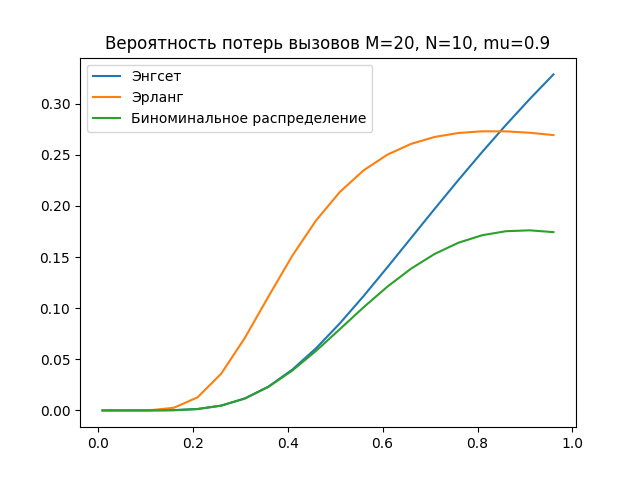
\includegraphics[scale=1.00]{assets/iss_1/loss_prob_M20_N10_mu09.png}
\caption{}
\label{}
\end{figure}

\begin{figure}[!htb]
\centering
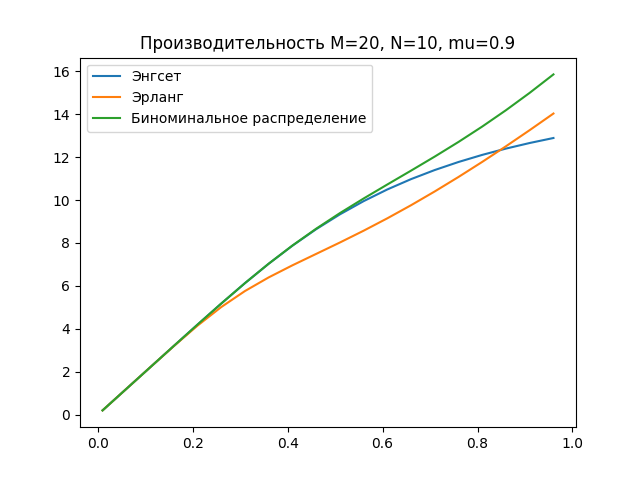
\includegraphics[scale=1.00]{assets/iss_1/perf_M20_N10_mu09.png}
\caption{}
\label{}
\end{figure}

\begin{figure}[!htb]
\centering
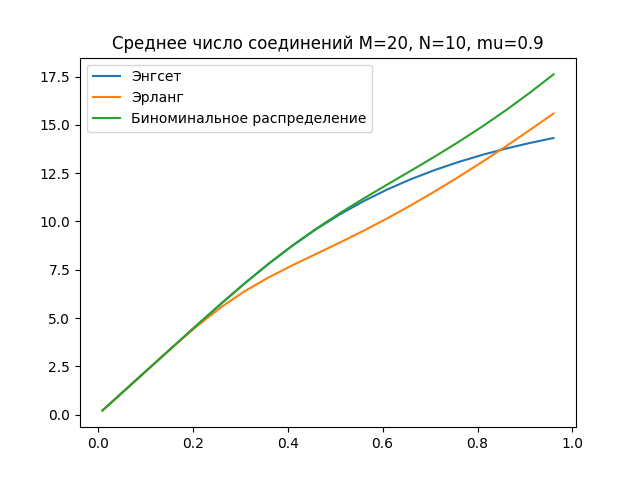
\includegraphics[scale=1.00]{assets/iss_1/aver_conn_M20_N10_mu09.png}
\caption{}
\label{}
\end{figure}

\subsection{$M ≫ N$}
\begin{figure}[!htb]
\centering
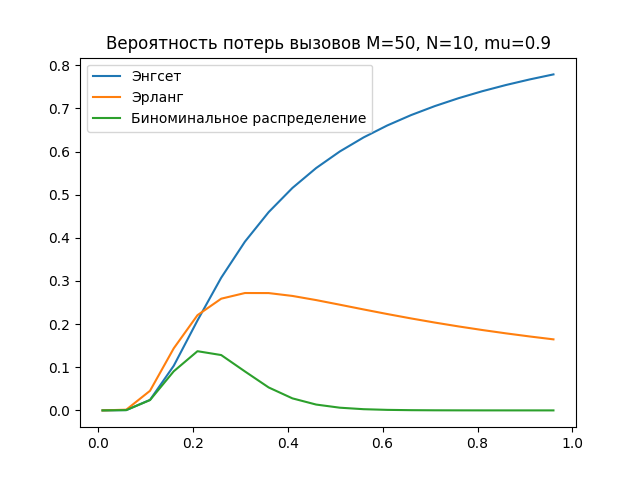
\includegraphics[scale=1.00]{assets/iss_1/loss_prob_M50_N10_mu09.png}
\caption{}
\label{}
\end{figure}

\begin{figure}[!htb]
\centering
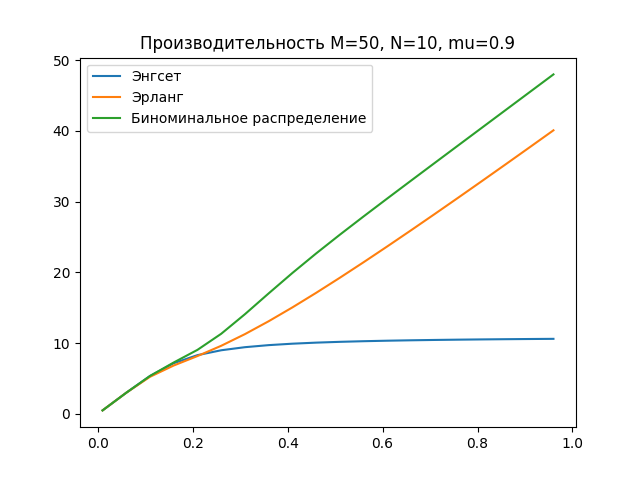
\includegraphics[scale=1.00]{assets/iss_1/perf_M50_N10_mu09.png}
\caption{}
\label{}
\end{figure}

\begin{figure}[!htb]
\centering
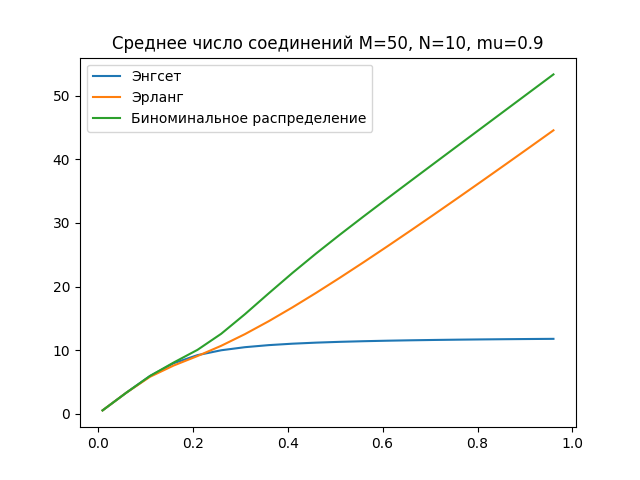
\includegraphics[scale=1.00]{assets/iss_1/aver_conn_M50_N10_mu09.png}
\caption{}
\label{}
\end{figure}

\subsection{Вывод}
При исследовании зависимости параметров коммутационной системы от интенсивности поступления нагрузки были получены следующие выводы:
\begin{itemize}
	\item При $M = N$:
	\begin{itemize}
		\item Наименьшая вероятность потерь вызовов с вероятностью поступления вызовов по распределению Эрланга или Биномиальному распределению
		\item Чем выше коэффициент интенсивности ухода потока нагрузки, тем лучше результат.
	\end{itemize}
	\item При $ M ≫ N$
		\begin{itemize}
			\item Наибольшая производительность системы
			\item Наиболее эффективный результат дает распределение Энгсета и Биномиальное распределение, $\mu$ при этом не имеет существенного влияния.
			\item Среднее число соединений в  системе также имеет наибольшее значение при наименьшем значении $\mu$, с подчинением закону распределения Энгсета и Биномиальному
		\end{itemize}
\end{itemize}

Параметры коммутатора во многом зависят от:
\begin{itemize}
	\item Закона распределения вероятностей поступающих заявок в систему
	\item $\lambda$
	\item $\mu$
	\item $\rho = \frac{\lambda}{\mu}$
\end{itemize}
Для каждого конкретного случая необходимо учитывать все эти характеристики в совокупности для получения требуемых параметров системы.

\section{Задача 2. Зависимость параметров от $\mu$}

\begin{figure}[!htb]
\centering
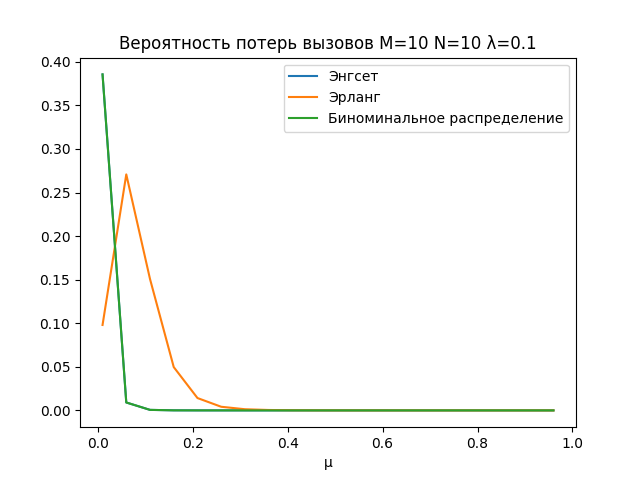
\includegraphics[scale=1.00]{assets/iss_2/loss_prob_M10_N10_lam01.png}
\caption{}
\label{}
\end{figure}

\begin{figure}[!htb]
\centering
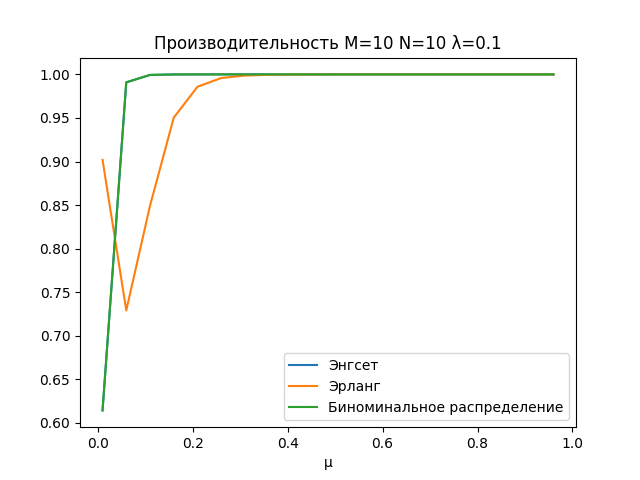
\includegraphics[scale=1.00]{assets/iss_2/perf_M10_N10_lam01.png}
\caption{}
\label{}
\end{figure}

\begin{figure}[!htb]
\centering
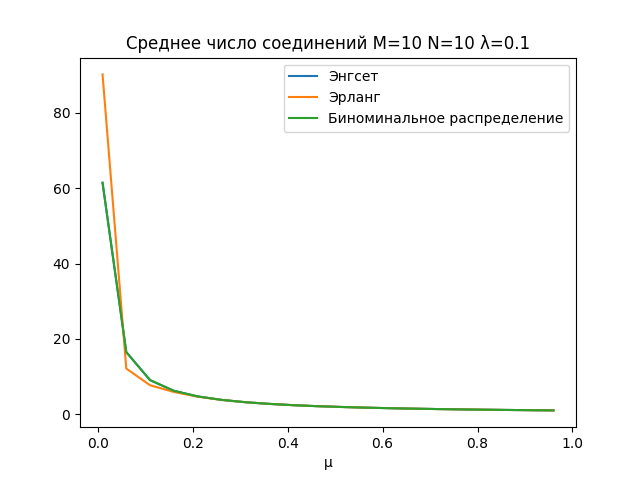
\includegraphics[scale=1.00]{assets/iss_2/aver_conn_M10_N10_lam01.png}
\caption{}
\label{}
\end{figure}

\subsection{$M > N$}\label{subsec2:}
\begin{figure}[!htb]
\centering
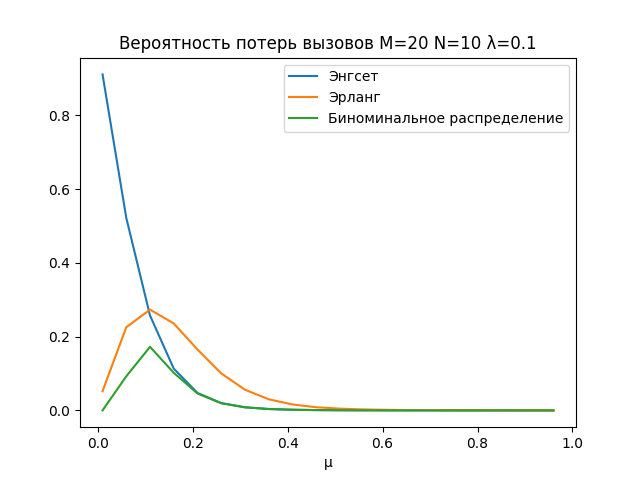
\includegraphics[scale=1.00]{assets/iss_2/loss_prob_M20_N10_lam01.png}
\caption{}
\label{}
\end{figure}

\begin{figure}[!htb]
\centering
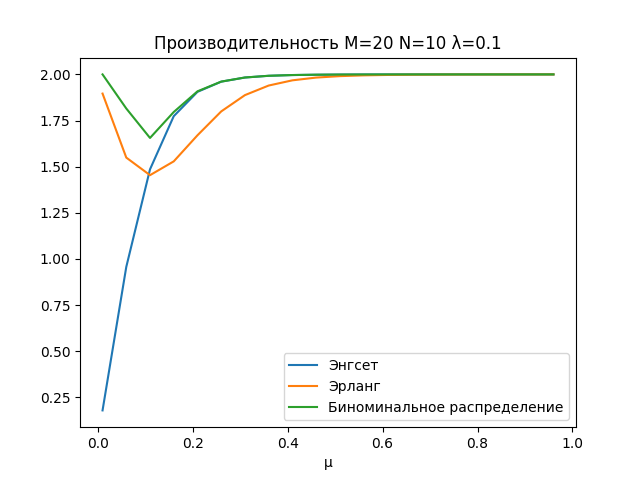
\includegraphics[scale=1.00]{assets/iss_2/perf_M20_N10_lam01.png}
\caption{}
\label{}
\end{figure}

\begin{figure}[!htb]
\centering
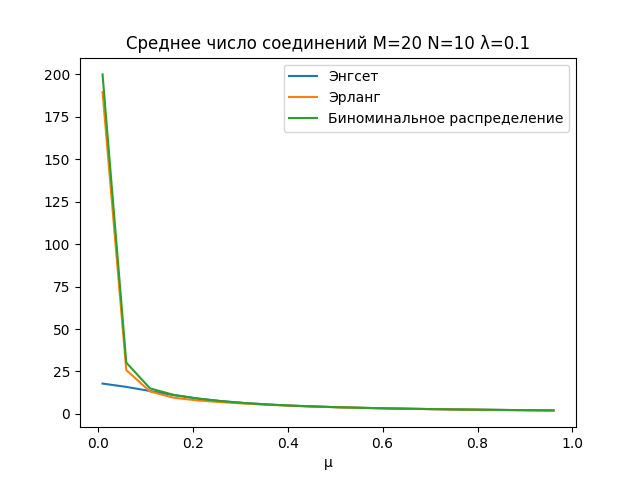
\includegraphics[scale=1.00]{assets/iss_2/aver_conn_M20_N10_lam01.png}
\caption{}
\label{}
\end{figure}

\subsection{$M ≫ N$}
\begin{figure}[!htb]
\centering
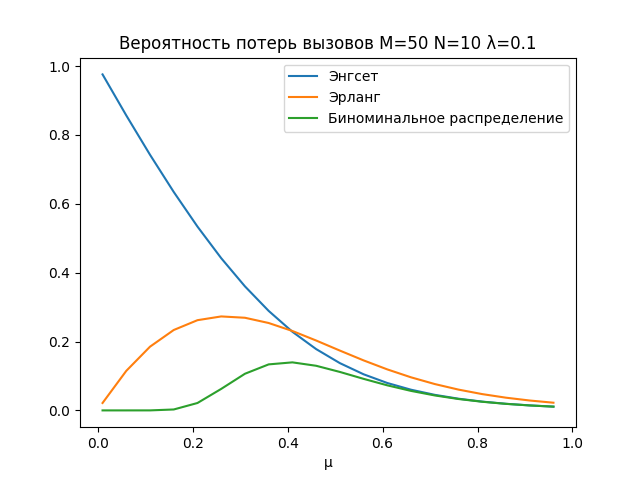
\includegraphics[scale=1.00]{assets/iss_2/loss_prob_M50_N10_lam01.png}
\caption{}
\label{}
\end{figure}

\begin{figure}[!htb]
\centering
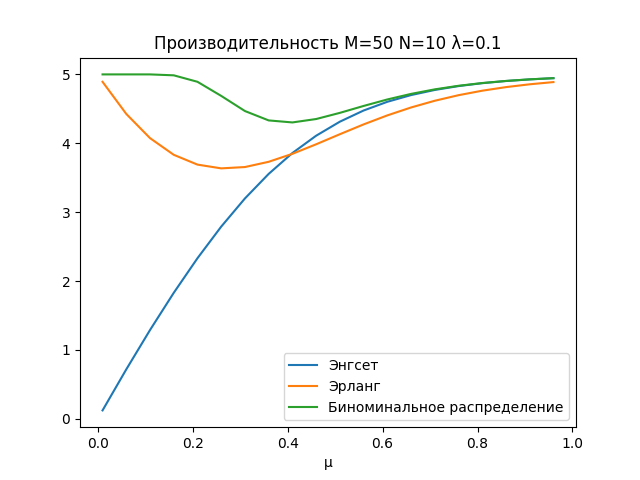
\includegraphics[scale=1.00]{assets/iss_2/perf_M50_N10_lam01.png}
\caption{}
\label{}
\end{figure}

\begin{figure}[!htb]
\centering
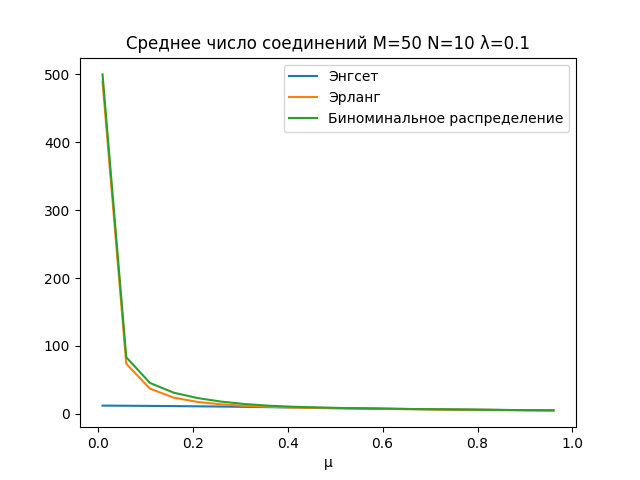
\includegraphics[scale=1.00]{assets/iss_2/aver_conn_M50_N10_lam01.png}
\caption{}
\label{}
\end{figure}

\subsection{Вывод}
Будет


\section{Задача 3. Зависимость параметров от $\rho$}
\subsection{$M = N$}
\begin{figure}[!htb]
\centering
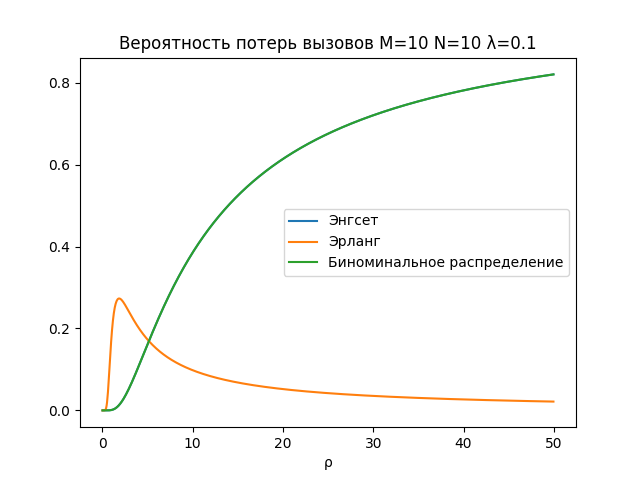
\includegraphics[scale=1.00]{assets/iss_3/loss_prob_M10_N10_lam01.png}
\caption{}
\label{}
\end{figure}

\begin{figure}[!htb]
\centering
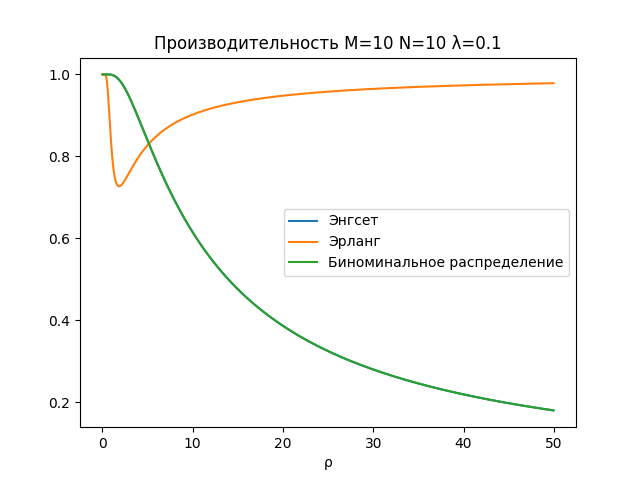
\includegraphics[scale=1.00]{assets/iss_3/perf_M10_N10_lam01.png}
\caption{}
\label{}
\end{figure}

\begin{figure}[!htb]
\centering
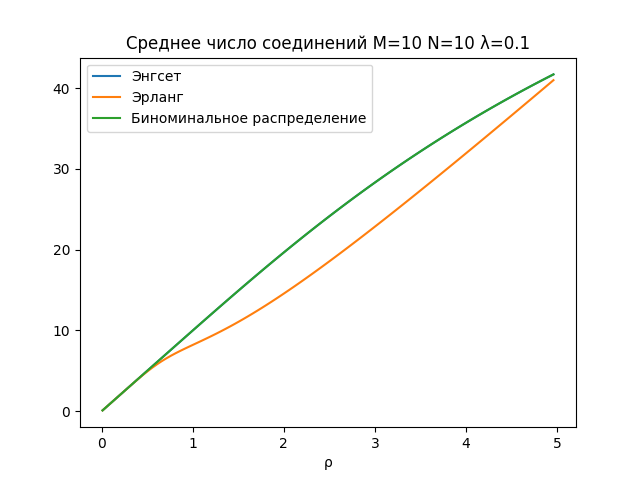
\includegraphics[scale=1.00]{assets/iss_3/aver_conn_M10_N10_lam01.png}
\caption{}
\label{}
\end{figure}

\subsection{$M > N$}\label{subsec2:}
\begin{figure}[!htb]
\centering
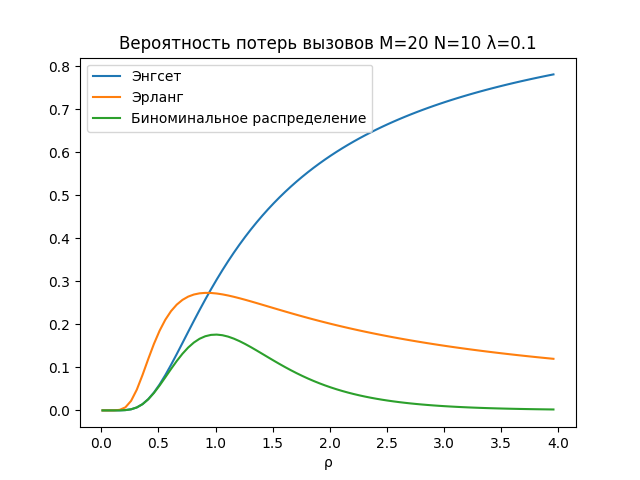
\includegraphics[scale=1.00]{assets/iss_3/loss_prob_M20_N10_lam01.png}
\caption{}
\label{}
\end{figure}

\begin{figure}[!htb]
\centering
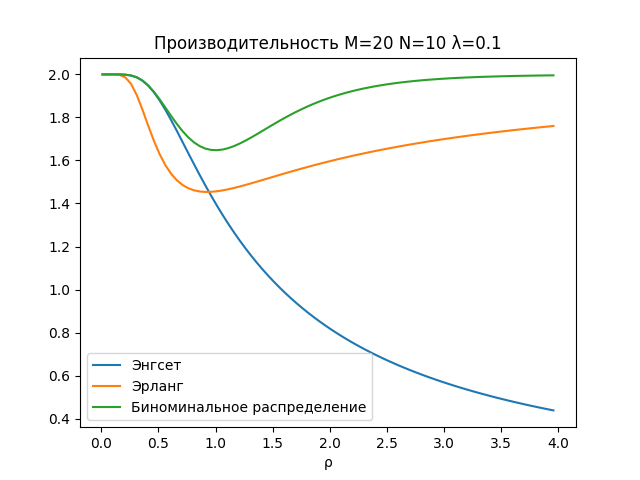
\includegraphics[scale=1.00]{assets/iss_3/perf_M20_N10_lam01.png}
\caption{}
\label{}
\end{figure}

\begin{figure}[!htb]
\centering
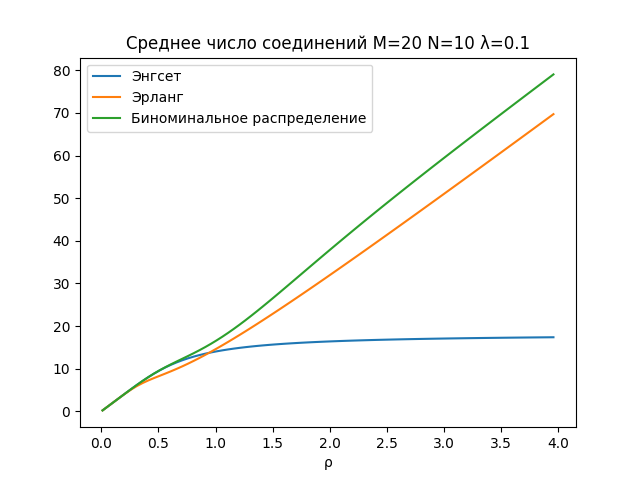
\includegraphics[scale=1.00]{assets/iss_3/aver_conn_M20_N10_lam01.png}
\caption{}
\label{}
\end{figure}

\subsection{$M ≫ N$}
\begin{figure}[!htb]
\centering
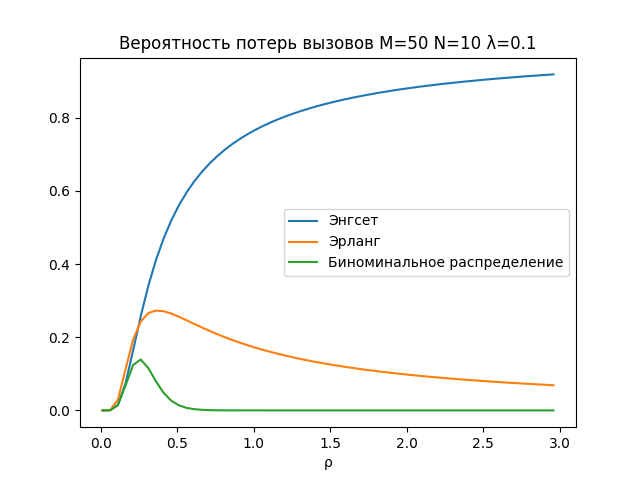
\includegraphics[scale=1.00]{assets/iss_3/loss_prob_M50_N10_lam01.png}
\caption{}
\label{}
\end{figure}

\begin{figure}[!htb]
\centering
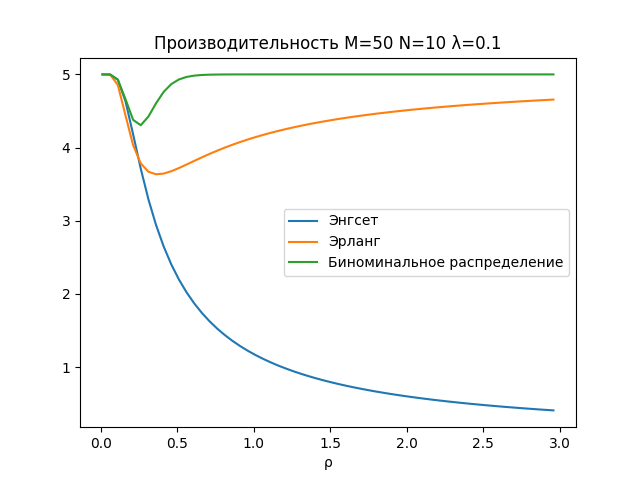
\includegraphics[scale=1.00]{assets/iss_3/perf_M50_N10_lam01.png}
\caption{}
\label{}
\end{figure}

\begin{figure}[!htb]
\centering
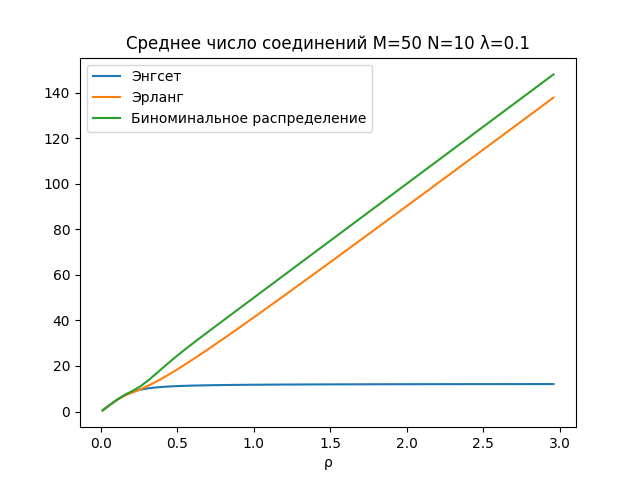
\includegraphics[scale=1.00]{assets/iss_3/aver_conn_M50_N10_lam01.png}
\caption{}
\label{}
\end{figure}

\subsection{Вывод}
Будет


\section{Задача 4. Зависимость параметров от $k = \frac{N}{M}$. Заменена зависимостью от $N$ при фиксированном $M$}
\subsection{$M = N$}
\begin{figure}[!htb]
\centering
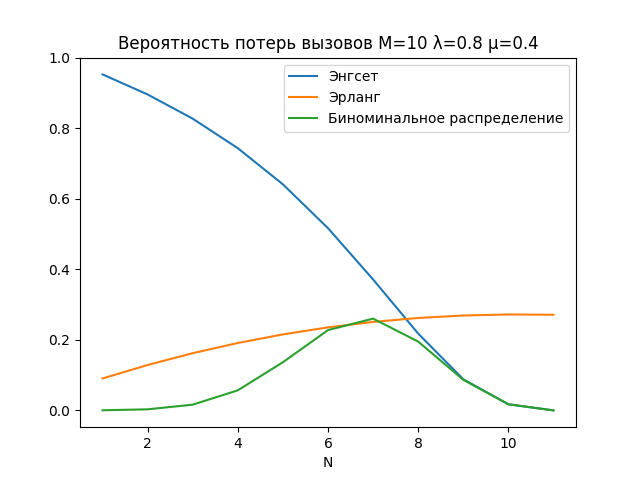
\includegraphics[scale=1.00]{assets/iss_4/loss_prob_M10_lam08_mu04.png}
\caption{}
\label{}
\end{figure}

\begin{figure}[!htb]
\centering
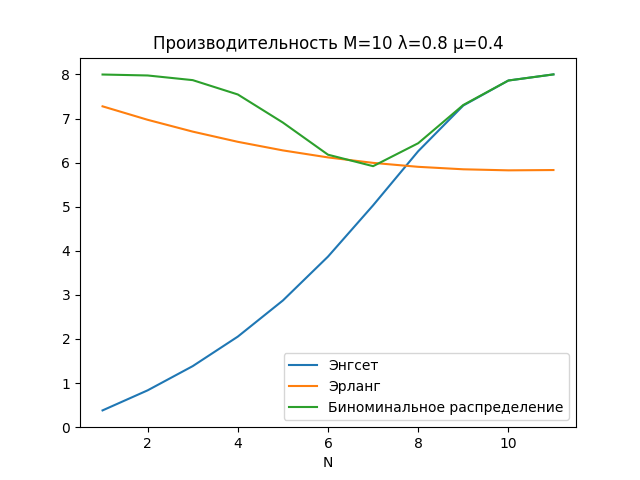
\includegraphics[scale=1.00]{assets/iss_4/perf_M10_lam08_mu04.png}
\caption{}
\label{}
\end{figure}

\begin{figure}[!htb]
\centering
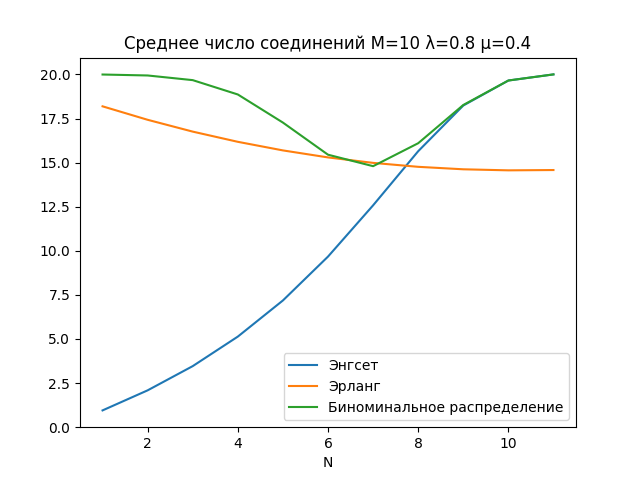
\includegraphics[scale=1.00]{assets/iss_4/aver_conn_M10_lam08_mu04.png}
\caption{}
\label{}
\end{figure}

\subsection{$M > N$}\label{subsec2:}
\begin{figure}[!htb]
\centering
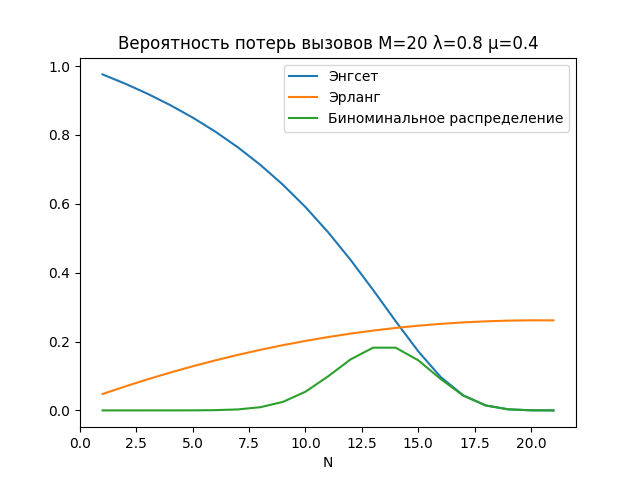
\includegraphics[scale=1.00]{assets/iss_4/loss_prob_M20_lam08_mu04.png}
\caption{}
\label{}
\end{figure}

\begin{figure}[!htb]
\centering
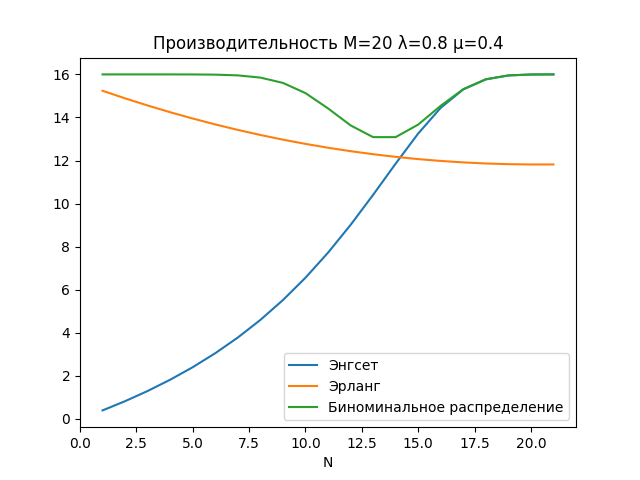
\includegraphics[scale=1.00]{assets/iss_4/perf_M20_lam08_mu04.png}
\caption{}
\label{}
\end{figure}

\begin{figure}[!htb]
\centering
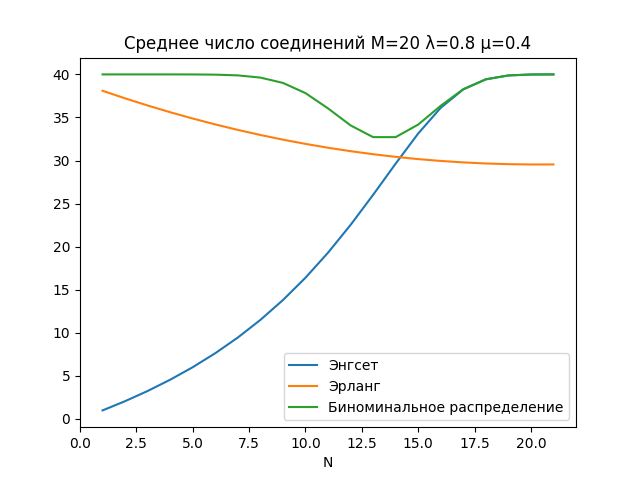
\includegraphics[scale=1.00]{assets/iss_4/aver_conn_M20_lam08_mu04.png}
\caption{}
\label{}
\end{figure}

\subsection{$M ≫ N$}
\begin{figure}[!htb]
\centering
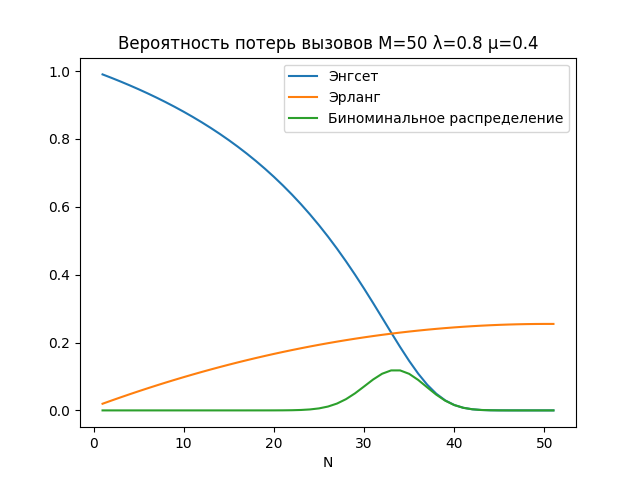
\includegraphics[scale=1.00]{assets/iss_4/loss_prob_M50_lam08_mu04.png}
\caption{}
\label{}
\end{figure}

\begin{figure}[!htb]
\centering
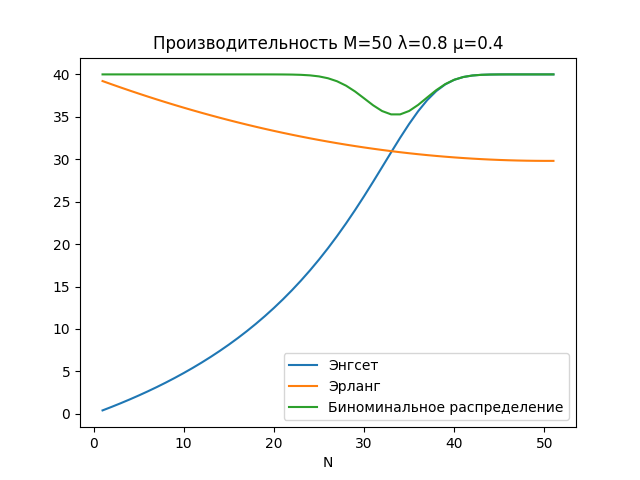
\includegraphics[scale=1.00]{assets/iss_4/perf_M50_lam08_mu04.png}
\caption{}
\label{}
\end{figure}

\begin{figure}[!htb]
\centering
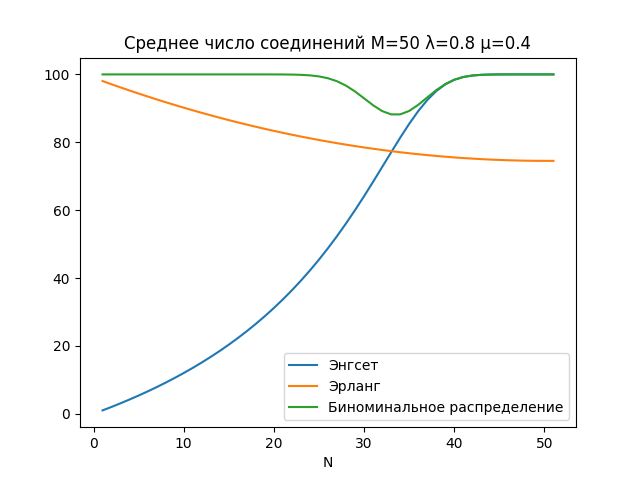
\includegraphics[scale=1.00]{assets/iss_4/aver_conn_M50_lam08_mu04.png}
\caption{}
\label{}
\end{figure}

\subsection{Вывод}
Будет


\end{document}